\documentclass[12pt]{ucthesis}

\usepackage{etex}
\usepackage[morefloats=125]{morefloats}
\usepackage[hyphens]{url}
\usepackage[breaklinks=true]{hyperref}
\usepackage{subfig}
\usepackage{graphicx}
\usepackage{tabularx}
\usepackage{amssymb}
\usepackage{amsmath}
\usepackage[letterpaper]{geometry}
\usepackage[overload]{textcase}
\usepackage{color}
\usepackage[nonumberlist,toc]{glossaries}
\usepackage{wrapfig}
\usepackage{longtable}
\usepackage{morefloats}
\usepackage{float}
\usepackage{listings}
\usepackage{makecell}
\usepackage[titletoc]{appendix}
\usepackage{cleveref}
\usepackage[]{algorithm2e}

\makeindex
\makeglossaries

\bibliographystyle{abbrv}

\setlength{\parindent}{0.25in} \setlength{\parskip}{6pt}
\geometry{verbose,nohead,tmargin=1in,bmargin=1in,lmargin=1.5in,rmargin=1in}
\setcounter{tocdepth}{2}

% Different font in captions (single-spaced, bold) ------------
\newcommand{\captionfonts}{\small\bf\ssp}

\newcommand{\mycaption}[2]{\caption[#1 --- #2]{#1 --- #2}}

\makeatletter  % Allow the use of @ in command names
\long\def\@makecaption#1#2{%
  \vskip\abovecaptionskip
  \sbox\@tempboxa{{\captionfonts #1: #2}}%
  \ifdim \wd\@tempboxa >\hsize
    {\captionfonts #1: #2\par}
  \else
    \hbox to\hsize{\hfil\box\@tempboxa\hfil}%
  \fi
  \vskip\belowcaptionskip}
\makeatother   % Cancel the effect of \makeatletter
% ---------------------------------------

% Define Appendix refs
\crefname{app}{appendix}{appendices}
\Crefname{app}{Appendix}{Appendices}

\begin{document}

% Declarations for Front Matter
\title{Laff-O-Tron: Laugh Prediction in TED Talks}
\author{Andrew Acosta}
\degreemonth{June} \degreeyear{2016} \degree{Master of Science}
\defensemonth{June} \defenseyear{2016}
\numberofmembers{2}
   \chair{Professor Foaad Khosmood, Ph.D. \linebreak Department of Computer Science}
   \othermemberA{Associate Professor Aaron Keen, Ph.D. \linebreak Department of Computer Science}
   \othermemberB{Professor Franz Kurfess, Ph.D. \linebreak Department of Computer Science}
\field{Computer Science} \campus{San Luis Obispo}
\copyrightyears{seven}


\maketitle

\begin{frontmatter}

% Custom made for Cal Poly (by Mark Barry, modified by Andrew Tsui).
\copyrightpage

% Custom made for Cal Poly (by Andrew Tsui).
\committeemembershippage

\begin{abstract}
Your abstract goes in here

\end{abstract}

\begin{acknowledgements}
\noindent
Thanks to:
\begin{itemize}
    \item Andrew Guenther, for uploading this template
    \item Paul Sanders and Loading Ready Run for inspiring the name
\end{itemize}

\end{acknowledgements}

\tableofcontents

\listoftables

\listoffigures

\end{frontmatter}

\pagestyle{plain}

\renewcommand{\baselinestretch}{1.66}

\chapter{Introduction}

\textit{``... Pleasure has probably been the main goal all along. But I hesitate to admit it, because computer scientists want to maintain their image as hard-working individuals who deserve high salaries. Sooner or later society will realize that certain kinds of hard work are in fact admirable even though they are more fun than just about anything else. (Knuth 1993)''} \cite{oneliners}

Computers are being used for amazing things. There are computers that can verify faces with sight, computers that can determine music by hearing it, and computers that react to touch. But, with all of these advancements, programmers have yet to provide computers with the most important, essential, and human sense: a sense of humor. This is a sense so complicated that, while we have hearing aids and glasses, nothing fixes a terrible sense of humor. But maybe modern technology can help.

Much work has been done in the field of computational humor, both in trying to understand and generate humor. Although there has been success in humor identification, it has always been directed at understanding specific kinds of jokes. For example, understanding if a sentence can be made into a ``That's What She Said'' joke\cite{twss} is great, but their technique only works for that specific kind of joke. One liner identification \cite{oneliners} and pun generators, although great achievements in the field of computational humor, still suffer from being about a specific form of joke, and thus are hard to apply outside of their scope.

Laff-O-Tron attempts to widen the scope of humor recognition beyond narrow joke structures by attempting to predict laughter in TED talks.

\section{Laugh Prediction}
Laugh prediction is the ability to, after a line is said, predict how likely it is that it will be followed by a laugh. In a sense, this is trying to identify whether something was a punchline of a funny joke, without needing to discover what the joke is or why it is funny. We believe this can be done by analyzing paragraph structure and word choice, as well as humorous stylistics.

\section{Applications of Laugh Prediction}
Laughter is an essential part of being human, and humor has been ingrained into our species no matter the culture. On a grand scale, an AI that is able to laugh at a correct time would be a major step towards creating a more human like AI. However, let's look at more immediate uses for laugh prediction as well.

When it comes to researching humor, laugh prediction will allow new perspectives on joke structure and design. This can provide new insight on the joke telling process. With some fine tuning, a user might be able to practice their delivery style on specific environments; such as wedding ceremonies or political speeches. 

Laugh prediction could be used to test if something will merit a laugh in fields like advertising. This is important, as the repercussions from poorly made jokes can be massive when it comes to major advertisements. However, this risk comes with high reward, as humorous commercials tend to be memorable.

Lastly, laugh prediction will be able to improve human computer interaction when it comes to vocal communication. It will make the computer appear more human, as it will appear to have a sense of humor. Adding humor into human computer interaction has been proven to improve people's opinions of it.\cite{Teaching}\cite{Multi-Humoroid} Imagine a world where you can tell Siri or Cortana a joke, and it would be able to laugh (or groan) accordingly. 

\section{Laff-O-Tron}
This work outlines an application, referred to as Laff-O-Tron, which attempts to predict when there will be laughter in a text script. Laff-O-Tron uses machine learning and natural language processing (NLP) to analyze the script, and make predictions after each line based off of the training scripts. Laff-O-Tron was trained using transcripts from TED Talks and was successfully able to predict laughter. We believe that with a different training corpus, Laff-O-Tron can be used to predict laughter or even applause in other environments such as political speeches.

\section{Why TED Talks?}
In order to train Laff-O-Tron, we needed data where the laughter had already been identified. Rather than manually adding laughter to scripts we already had, we decided to find new scripts that already had laughter marked down. After a thorough investigation, we found that TED Talk transcripts had audience laughter already marked, and decided to use them as our data. This design choice greatly impacts how Laff-O-Tron works, as environment has an incredible impact on humor. The kind of humor that is prevalent in bars, for example, is different than the humor found at a wedding. Thus, Laff-O-Tron is designed to predict laughter in a live talk environment. 


\section{Contribution}
The goal of this project was to show that it is possible for a computer system to be able to predict laughter without needing depending on a narrow joke structure such as knock knock joke or pun. Although Laff-O-Tron was a success, more research needs to be done to generalize this beyond TED Talks. 

This project has also contributed to the field of NLP as a whole by creating a corpus of TED Talks, free to use by anyone.

\chapter{Background}

Laugh prediction is a topic that falls under the humor recognition part of computational humor. Humor recognition has employed multiple algorithms and methods in order to determine what is humorous and what is not. This is a complicated problem as one man's laugh can be another man's groan. Despite this, people have had success working on systems from detecting one-liners to identifying knock knock jokes. These achievements are possible thanks to the fields Computational Linguistics and Machine Learning. 

Since computational humor is part of the broader field of computational linguistics, we will take a quick look at that first.


\section{Computational Linguistics}
``Human knowledge is expressed in language. So computational linguistics is very important.''–Mark Steedman, ACL Presidential Address (2007) \cite{comp_ling}

Computational linguistics is an interdisciplinary field concerned with understanding written and spoken language from a computational perspective and building artifacts that can process and produce language. \cite{comp_ling} Our method for laugh prediction in particular is concerned with parsing and understanding text. To parse text, we need to break it up into tokens using a method called tokenizing.

\begin{figure}
\centering
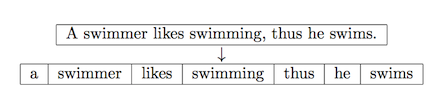
\includegraphics{figures/tokenizing}
  \caption{Example of tokenizing a sentence. \cite{ngrams}}~\label{fig:tokenizing}
\end{figure}

Tokenizing by words can be thought of as splitting the text into individual words and ignoring all white space. Punctuation is handled differently, based on what the programmer wants. An example can be seen in figure \ref{fig:tokenizing}. As you can see, there is a token for each word in the sentence and the spaces are ignored. The tokenizer we used treats punctuation as their own words, while the tokenizer in in figure \ref{fig:tokenizing} chooses to ignore them. One can also tokenize by characters instead of words.

Once we tokenize the text, we can break the tokens up into N-grams in order to analyze it. N-grams are just collections of N tokens put together to be looked at. An example can be seen in figure \ref{fig:ngrams}. Compared to the tokenization picture, you can see that the unigram (1-gram) chunk is just the sentence tokenized. In the bigram (2-gram) chunk, each bigram is a pair of words that are next to each other. As you can see, the same word shows up in 2 bigrams: one with the previous word and one with the next word. The trigrams (3-grams) chunk shows how each trigram is a triple of words that works like the bigrams above it. As mentioned above, N-grams are based on the tokens provided, meaning that the way we tokenize text determines the N-grams that we analyze.

\begin{figure}
\centering
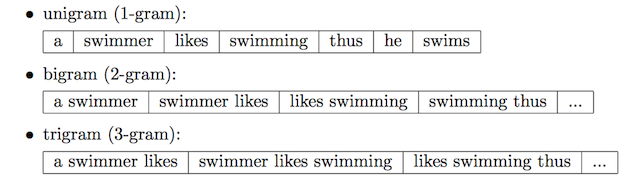
\includegraphics[width=.7\columnwidth]{figures/ngram}
  \caption{Example of breaking up a sentence with N-grams. \cite{ngrams}}~\label{fig:ngrams}
\end{figure}

Beyond parsing, we looked at what percent of the words in each paragraph are nouns, verbs, and adjectives. We were able to do this using a Parts of Speech (POS) tagger. A POS tagger looks at a word and tries to decide what kind of word it is. For example, it might guess that ``homework'' is a noun, and ``dreading'' is a verb. With this, all we had to do was put our tokens through the tagger, and it will tag each token with its respective POS. 

\subsection{Natural Language Toolkit}
We used the Natural Language Toolkit (NLTK) python library for POS tagging, tokenizing strings, and creating N-grams. We also took advantage of its built-in classifiers: Naive Bayes, Decision Trees, and Maximum Entropy. NLTK is an open source library that includes ``extensive software, data, and documentation'' related to the field of Natural Language Processing (NLP).\cite{NLTK} Originally created back in 2001 at the University of Pennsylvania, it has developed into an easy to use library that allows users to dive into NLP without much experience. NLTK works with Python 2 and 3, and can easily be downloaded on their website: http://www.nltk.org/. \cite{NLTK}

\section{Computational Humor}
\textit{``Computational humor is a branch of computational linguistics and artificial intelligence which uses computers in humor research. It is not to be confused with computer humor (i.e., jokes about computers, programmers, users, and computing).''} (Wikipedia)

Computational humor is a relatively new area, with the first dedicated conference organized in 1996 \cite{conference}. This conference was last held again in 2012.

``Work on computational humor can be divided into two classes: humor recognition and humor generation.'' \cite{xyz} Humor generation is the more commonly seen of the two. One of the earliest implementations of humor generation dates back to 1992 with a pun generator.\cite{Lessard} Since then, not only have more pun generators been made, but other flavors of joke generators have been created as well. Here is an example of a pun generated by the software STANDUP, originally designed to teach children about the English language.

``What do you call a nauseous tree?''

``A sick-amore!'' \cite{STANDUP}

Joke generators have stuck to jokes with pre-built structures. Instead of generating whole sentences, they just fill in the blanks. This is still very impressive, as it means that the AI understands humor enough to utelize these structures in a humorous way.

Although there has been much work on humor recognition, it is often seen as the harder of the two since humor generation gets the luxury of using the structures previously mentioned. \cite{metatheory} To make up for this, machine learning classification models have been used to find the differences between humorous and non-humorous text. Unfortunately, this has led to humor recognition to be designed only for specific structures of humor. For example, one-liner detection is humor recognition that works only on the one liner structure. This means that jokes that don't utilize this structure will go over this system's metaphorical head. The same is true with a method designed to tell if something is a knock knock joke. Although these are still very impressive, it is important to note that they focus on what the differences between a humorous and non-humorous text are, and not why the text itself is humorous.

\section{Humor Theory}
Humor theory is an age old field that has been traditionally divided into three branches. These are not all the branches, but only the basic traditional branches. ``Most of the humor theories ever proposed are actually mixed theories, and many contemporary researchers believe that humor in its totality is too huge and multiform a phenomenon to be incorporated into a single integrated theory.'' \cite{humor_theory} 

\subsection{Theories of Incongruity, Inconsistency, or Contradiction} 
Incongruity can be defined as the state of being out of place. Thus, these theories focus more on some objective or characteristics of a humorous text or act. This objective or characteristic seems out of place or unexpected; it seems to contradict the whole. Because of this, this branch of humor theory is more on a cognitive level.

This theory assumes that every humorous act involves two frames of reference that are mutually incompatible, but share a common part. This common part allows someone to shift from one frame to another. This causes the recipient to follow the first frame of reference, maintaining that interpretation until the shift to the second frame occurs and the interpretation fails. This is when some cognitive work occurs allowing the interpretation to shift to the second frame of reference. It is believed then that ``the renewal of understanding is attended by the emotion of surprise and satisfaction, causing the reaction of laughter.'' \cite{humor_theory}. Below is an example that follows this branch of humor theory:

An English bishop received the following note from the vicar of a village in his diocese: ``Milord, I regret to inform you of my wife's death. Can you possibly send me a substitute for the weekend?''\cite{humor_theory}

\subsection{Theories of Superiority, Disparagement, or Criticism}
This theory addresses the alleged aggressive characteristic of laughter. This is ``humor [that] is said to be pointed against some person or group, typically on political, ethnic or gender grounds.'' Although this branch of humor may seem to be more hostile and destructive, this does not mean that this branch of humor is objectively bad. Insulting others using the cooperative principle of joke-telling can be used to for a social intimacy between all involved. This can be seen when a group of coworkers poke fun at a dictatorial boss. It can also be used to criticize someone or the state of something. The example below is designed to criticize lawyers:

``Criminal lawyer is a redundancy'' \cite{oneliners}

\subsection{Theories of Release, Relief, or Relaxation}
This branch of theories focuses more on the psychological effect of humor on the recipient. These effects are generally thought of as a way to convert stress or socially taboo aggressive impulses into something that is more socially accepted. This can be seen when someone is angry or stressed out about a subject, so they make jokes to make them feel better.


\section{Machine Learning}
\textit{``Machine Learning is a natural outgrowth of the intersection of Computer Science and Statistics''} \cite{machine_learning}

Machine learning tries to answer the question: ``How can we build computer systems that automatically improve with experience'' \cite{machine_learning}. Algorithms attempt to accurately predict certain characteristics of data by analyzing past sample data and generating models from it. We used the supervised learning method, which involves training the AI on data that has already been labeled. Our data specifically is labeled as laugh worthy or not. Another method for machine learning is the unsupervised learning method. Unsupervised learning involves the AI generating models with data that was initially, and then labeling the data itself. The goal for both of these methods is to create a system that can label new data correctly, as shown in figure \ref{fig:machinelearning}. Supervised learning is more often used for classification, which is why we chose to use that. \cite{machine_learning}

\begin{figure}
\centering
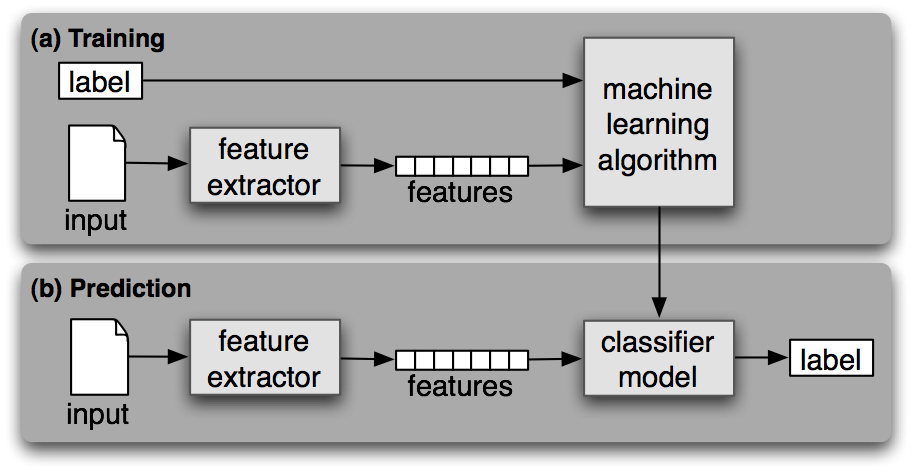
\includegraphics{figures/supervised-classification}
  \caption{Supervised Classification Visualization.\cite{NLTK}}~\label{fig:machinelearning}
\end{figure}

We chose to implement machine learning since it is an effective method for solving problems that are too complex to manually design algorithms for. \cite{machine_learning} Trying to make an algorithm for humor seems impossible to get right. Machine learning algorithms provided a way for us to get accurate results without needing to have a perfect algorithm. Once we decided to utilize machine learning, we needed to pick which machine learning classifiers to use. Classifiers are the algorithms that are trained and then used to classify new data. 

\subsection{Naive Bayes Classifier}
The Naive Bayes classifier is seen as the baseline classifier as it is the simplest. It trains by going through feature sets with matching classifications and finding the probability of each feature being associated with each classification. For testing, it goes through a feature set and chooses the most probable classification based on the presence or absence of the features. It is called naive because it assumes that all features are independent of other features. \cite{NLTK}
 
Let's look at an example where we were trying to figure out the genre of an article based off of the words using Naive Bayes. We would use the words in the article as the feature set, and the genres as the classifications. To determine the genre of the article, Naive Bayes will go through each feature (word) in its feature set. At each feature, it will attempt to see what genres that feature is most associated with and increase those genre's probability. It will also look at which words are significant but are not in the text, and adjust the probability accordingly. Figure \ref{fig:bayes} shows an example where the words ``dark'' and ``football'' appear in the text. ``Dark'' is often associated with the ``Murder Mystery'' genre, but it can appear in the other genres.\cite{NLTK} So it increases the probability of ``Murder Mystery'' slightly by moving the dot closer to it. But ``football'' is almost always used in the ``Sports'' genre, so the probability of ``Sports'' greatly increases. 
 
 \begin{figure}
\centering
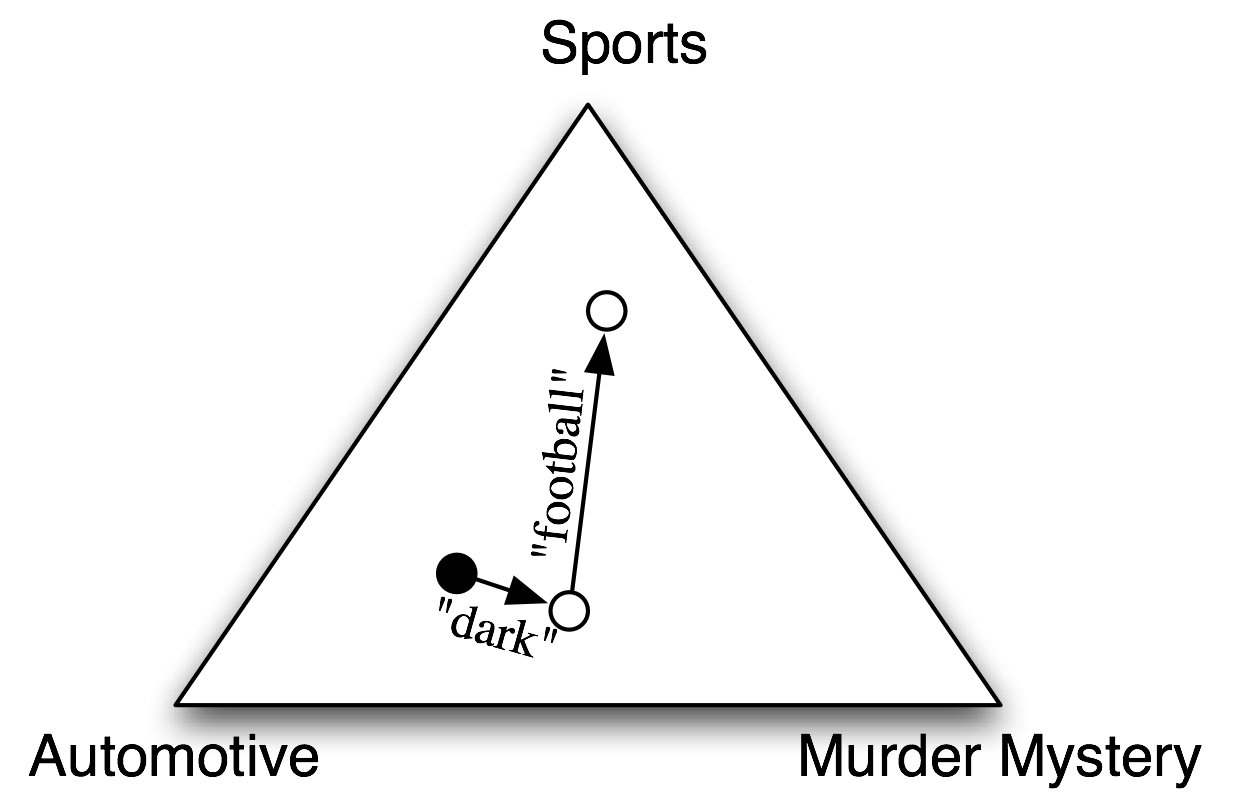
\includegraphics{figures/naive-bayes-triangle}
  \caption{An abstract illustration of the procedure used by the naive Bayes classifier to choose the topic for a document.\cite{NLTK}}~\label{fig:bayes}
\end{figure}


\subsection{Decision Tree Classifier}
The Decision Tree classifier is another machine learning method that can be used for classification. Like Naive Bayes, decision trees need to use supervised learning. This means that you must train it with pre-classified feature sets. \cite{NLTK}

 \begin{figure}
\centering
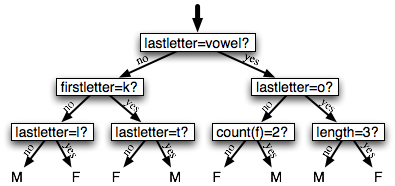
\includegraphics{figures/decision-tree}
  \caption{Decision Tree model for the name gender task.\cite{NLTK}}~\label{fig:dtree}
\end{figure}

The tree contains decision nodes and leaf nodes. Figure \ref{fig:dtree} shows a decision tree that is used to classify a name as either a male name or a female name. The decision nodes check the features being passed into the tree. In figure \ref{fig:dtree}, these would be nodes like ``first letter = k'' and ``last letter = vowel''. Based off if the decision node is true or false, the tree will go down to the next decision node or leaf node. The leaf nodes are what classify the object. In figure \ref{fig:dtree}, this can be seen as the ``m'' for male name and ``f'' for female name at the bottom of the tree. \cite{NLTK}

Decision trees have the advantage of being relatively simple to understand and are well suited for any problem with many hierarchical organized decisions. However, they do have some disadvantages. Because the decision tree splits the training data to create the nodes, the amount of data used to train some of the lower nodes becomes quite small. This means that the nodes on the bottom might be trained with such a small portion of the training data that they overfit the training set.\cite{NLTK} Overfitting a training set means that the decision tree learns ``patterns that reflect idiosyncrasies of the training set rather than linguistically significant patterns in the underlying problem.''\cite{NLTK} Overfitting can be minimized by pruning away the decision nodes that don't help improve the accuracy of the tree.

\subsection{Maximum Entropy}
Maximum Entropy is a machine learning method for classification that uses a model that is similar the the one used by Naive Bayes. However, Maximum Entropy uses search techniques to find a set of parameters that will maximize the performance of the classifier, instead of using probabilities to set the model's parameters. To do this, it chooses the model parameters using iterative optimization techniques, which initializes the model's parameters to random values and then repeatedly refines them to bring them closer to the optimal solution.\cite{NLTK}

Although more powerful than Naive Bayes on average, Maximum Entropy can take a very long time to run due to its iterative approach. Users should keep this in mind when their training sets, their number of features, and their number of labels are large.\cite{NLTK}

\subsection{Boosting}
Boosting is an approach to machine learning based on the idea that a strong and highly accurate predictor can be created from multiple weak and inaccurate predictors. ``Boosting solves hard machine-learning problems by forming a very smart committee of grossly incompetent but carefully selected members.'' \cite{boosting} One of the requirements of boosting is that the weak predictors are at least slightly better than random guessing. Boosting algorithms then run through the training data with the classifiers, noting what each classifier misses and adjusting how much it weighs each classifier's decision on certain features. For example, if classifier A is really good at predicting data that has Z features compared to the other classifiers, than A's classification would have more weight when predicting data with Z features. This way, when running the algorithm on new data, it attempts to play on the strengths of each classifier to improve their total value. 

We chose to use boosting because we managed to produce decent results using the classifiers listed above (Naive Bayes, Max Entropy, and Decision Trees). Each classifier had varying accuracy when exposed to different feature sets. Naive Bayes performed well, for example, when only looking at the words in the segment but did terrible when looking at the N-grams. Decision trees however did well when looking at N-grams and POS tagging. Max Entropy did very well when looking at all three at once, but took an exceptionally long time. Despite our results, all of these classifiers are still weak and not accurate enough. We then chose to use boosting believing that if we used these weak classifiers with boosting to create a strong classifier then our accuracy would improve significantly.

\chapter{Related Works}

Humor detection and laugh prediction are small areas in the field of computational linguistics. This is a result of computational humor being seen as more experimental, with its contributions being seen more in toys than in industry. Despite this, significant work has been done by researchers to try and identify laugh worthy and humorous text.

\section{One-Liners}
Mihalcea and Strapparava were some of the first to attempt to use computational humor for humor detection. They created a detector for one liners such as ``Take my advice, I don't use it anyway''.\cite{oneliners} The results were impressive, with accuracies of 84.82\% and 96.95\% when trying to identify humorous one liners from non-humorous proverbs and news article headlines respectively. This is particularly interesting because it is able to use the context held within the one line to identify if there is a joke. \cite{oneliners}

To detect if something is funny, the system looks at humor-specific stylistic features and at the content of the statement. \cite{oneliners} They used a machine learning approach similar to the one described in this paper to attempt to detect humor from their content. Their results using content based analysis alone was incredibly high, but when the humor-specific stylistics were added, the increase was statistically significant. So let's take a look at what stylistics they observed.

First, they decided to look at the stylistic feature of alliteration. This is because ``one-liners often rely on the readers' awareness of attention-catching sounds, through linguistic phenomena such as alliteration, word repetition, and rhyme, which produce a comic effect even if the jokes are not necessarily meant to be read aloud.'' \cite{oneliners} This is not a trend in just one-liners however, studies found that the ``phonetic properties of jokes are at least as important as their content.'' \cite{oneliners} Alliteration turned out to be the most useful indicator of humor of all the humor-specific stylistic features. Below are two examples of one-liners with their alliteration underlined:\newline

``\underline{V}eni, \underline{V}idi, \underline{V}isa: \underline{I} came, \underline{I} saw, \underline{I} did a little shopping.'' \cite{oneliners}

``\underline{Infan}ts don’t enjoy \underline{infan}cy like \underline{adult}s do \underline{adult}ery.'' \cite{oneliners}\newline

They then looked at antonymy in the statement. This is because ``humor often relies on some type of incongruity, opposition, or other forms of apparent contradiction'' \cite{oneliners} Unfortunately, accurate identification of all these properties is too difficult to accomplish. So Mihalcea and Strapparava decided to just look at the presence of antonyms in the statement. They also looked at indirect antonymy by checking if the synonyms of the words had antonyms. Unfortunately, this was not fully complete, which may have been why antonymy did not perform too well. Although it did help identify one-liners, it was nowhere near as useful as alliteration. However, it did do better than their next humor-specific stylistic feature.\cite{oneliners} Below are two examples of one-liners with their antonymy underlined:\newline

``A \underline{clean} desk is a sign of a \underline{cluttered} desk drawer.''\cite{oneliners}

``Always try to be \underline{modest} and be \underline{proud} of it!''\cite{oneliners}\newline

Adult slang was the last stylistic feature they used. This checked to see if adult slang such as ``sex'' and ``procreation'' was present. To do this, they had their system detect sexual-oriented words. This was the least useful feature, but it did help when identifying one-liners.\cite {oneliners} A later experiment used a similar approach to detect when a ``that's what she said'' joke could be made.\cite {twss} Below are two examples of one-liners with their adult slang underlined:\newline

``The \underline{sex} was so good that even the neighbors had a cigarette.''\cite{oneliners}

``Artificial \underline{Insemination}: \underline{procreation} without recreation.''\cite{oneliners}

\section {Knock Knock Joke Recognition}
Of all the jokes an AI could recognize, one would expect a knock knock joke to be the easiest. There is a simple structure to look for, so it would make sense to end it there. Unfortunately, it is not that easy, as Taylor and Mazlack found out. They created a system that was designed to identify knock knock jokes. \cite{knockknock} To do this they had to look beyond the structure to see if what was said was really a joke or not. Their system needed to check if there was a funny punchline, or it would not be considered a joke. They tested their system with a corpus of real and fake knock knock jokes. The fake jokes had coherent last lines, but they were not actually punchlines. In this example, the first joke is a real knock knock joke, while the second is a fake:\newline\newline
``Joke 6: Knock, Knock \newline
Who's there?\newline
Justin\newline
Justin who?\newline
Justin time for dinner.\newline\newline
Text1: Knock, Knock\newline
Who's there?\newline
Justin\newline
Justin who?\newline
Justin awoke in the middle of the night.'' \cite{knockknock}\newline\newline
The system was able to recognize 69\% of the jokes it was given as real. Furthermore, it was able to recognize 95\% of the fake jokes as such. Although it still needs more work, it was a major step in humor recognition.

\section{Double Entendre Detector}
In a similar vein to laugh prediction, Kiddon and Brun created a system for predicting if ``That's what she said'' should be said after a sentence. In 2011, they created a system called DEviaNT that is able to detect if a sentence has enough double entendres necessary to add ``That's what she said'' to the end of the sentence. They did so by looking at the words used and the structure of the sentence. This is because ``That's What She Said Jokes'' (TWSS) are ``likely to contain nouns that are euphemisms for sexually explicit nouns and… share common structure with sentences in the erotic domain.'' \cite{twss}

When looking at the words in the sentence, their system analyzed the sexiness of each word. This means that the presence of sexy words like ``hot'' or ``wet'' would increase the likelihood of it being a TWSS. In order to do this, they trained an AI using their erotica corpus for erotic text, and the Brown corpus for non-erotic text. This allowed the AI to measure the sexiness of words. For detecting the structure of a TWSS, they looked at the amount of punctuation, pronouns, and subjects in the sentence. 

Although this is focused on predicting TWSS, this has some connections to our work as well. The way they looked at structure in a TWSS is similar to how we looked at the structure of a segment to determine if the audience would laugh or not. Unfortunately, we chose not to measure the sexiness of each word, but instead how often that word was used in segments that caused laughter. Although two different measurements, there are probably many words that would rank highly in both of our systems.


\chapter{System Evaluation}

The goal of this system is to be able to accurately predict when laughter would show up in a TED talk. This goal entails both correctly predicting a laugh when one would occur, and not predicting a laugh when one wouldn't occur. To test this, we trained our system using approximately 80\% of the TED talk data we had collected, and then tested it against the other 20\% of the TED talk data which it had never seen before. 

We then looked at three different measures to determine its overall accuracy: precision, recall, and F-measure. Precision ``indicates how many of the items that we identified were relevant...''\cite{NLTK}. This can be thought of as ``What percent of positives were true positives?'' Recall ``indicates how many of the relevant items that we identified…''\cite{NLTK}. Another way to look at this is ``What percent of all of the positives did we correctly identify?'' Finally, F-measure ``combines the precision and recall to give a single score''\cite{NLTK}. It is defined as:

	(2 * Precision * Recall) / (Precision + Recall)

Lastly, we looked at the effects of adding in certain humorous stylistics to search for. 

\section{Data Collection}
We used the transcripts of XX (TODO) TED Talks scraped from the TED website. We then limited the talks by length of the script in order to remove any songs or extremely short TED talks that would show up. This is important because songs are not the type of talks we are looking for. Talks with incredibly small scripts are not helpful either, as they are focused on something unseen, which cannot be captured by the transcript well.

\section{Evaluation}
To evaluate the system, we first went through each TED talk and broke it up by paragraph. We skipped paragraphs that were just applause. Then, if a laugh was recorded in the paragraph or immediately after the paragraph (which was more often the case), the paragraph would be considered Laughter Positive. Otherwise it was marked Laughter Negative. The laughs themselves were also removed from the paragraphs. Next, 80\% of the paragraphs was used to train the system to correctly identify a Laughter Positive paragraph. Finally, the remaining 20\% of the paragraphs were used to test the system’s accuracy.  

This process was done for several versions of the system, each using different classifiers and feature sets, as well as looking for humor specific stylistics.


\section{Analysis}
TODO! State and analyze results here



\clearpage
\begin{flushleft}
\nocite{*}
\bibliography{bibliography}
\bibliographystyle{plain}
\end{flushleft}

\begin{appendices}


\end{appendices}

\end{document}
